\documentclass[10pt,letterpaper]{article}

\usepackage{ccn}
\usepackage{pslatex}
\usepackage{apacite}
\usepackage{graphicx}
\usepackage{caption}
\usepackage{natbib}
\usepackage{float}

\usepackage{hyperref}
\usepackage{url}
\usepackage{booktabs}
\usepackage{amsfonts}
\usepackage{nicefrac}
\usepackage{microtype}
\usepackage{xcolor}
\usepackage{amsmath}
\usepackage{amssymb}
\usepackage[labelfont=bf, margin=0.8cm, font=sf]{caption}

% DRAFT generated from results/ on 2026-10-17. Numbers come from results/C1/headline.json,
% results/C1/gate_attribution.csv, results/B1/fertility.csv and results/B2/lm_2x2.csv.
% Re-check every number against those files after any re-run.

\title{Erased and Penalised: 19th-Century isiXhosa Newspapers in a Modern LLM Data Pipeline}

\author{{\large \bf Sunay Master (2677874)}
  \AND {\large \bf Matthew Purkiss (2697424)}
  \AND {\large \bf Harshil Vallabh (2656158)} }

\begin{document}

\maketitle
\phantom{.}
\newpage
\phantom{.}
\newpage

\section{Abstract}
{
\bf
\looseness=-1
Large language models are trained on text that survives filter cascades tuned on English web data. We ask what happens to the earliest African-edited isiXhosa journalism when it meets such a pipeline, and how much of the damage is due to its pre-reform spelling rather than to genuine linguistic or cultural difference. We pass 150-word windows of \emph{Isigidimi samaXosa} (1870--1888) and \emph{Imvo Zabantsundu} (1884--1894) through re-implementations of four standard gates (language ID, Gopher quality rules, the C4 bad-words list, CCNet perplexity), alongside modern isiXhosa news and the English columns printed on the same pages. None of 5{,}000 historical isiXhosa windows survives, against 32.6\% of the English columns. Language ID is not the problem (95\% recognised as isiXhosa); the English stop-word rule removes 96\% of \emph{all} isiXhosa, modern or historical, and the perplexity gate removes 100\% of the historical text but 72\% of modern news. A transparent spelling normaliser closes 26\% [22, 29] of the perplexity gap but leaves survival at zero; tokenisers charge isiXhosa 1.1--1.6$\times$ more tokens per letter than English yet barely distinguish 1880s from modern spelling. The bad-words list mainly removes surnames, seed advertisements and the period spelling of \emph{namhla} (``today'').
}
\begin{quote}
\small
\textbf{Keywords:}
pretraining data filtering; historical text; isiXhosa; orthography; representational harm
\end{quote}

\section{Introduction} \label{Intro}
\looseness=-1
Pretraining corpora are not samples of language but the output of curation: language identification (LID), heuristic quality rules \citep{rae2021gopher}, word blocklists \citep{raffel2020c4} and perplexity filters against a reference corpus \citep{wenzek2020ccnet}. Audits show these steps disproportionately remove minority-identity and dialectal English \citep{dodge2021c4} and that multilingual web corpora for low-resource languages are often of poor quality \citep{kreutzer2022quality}. We study a case where the text is of high cultural value and the language is low-resource: the isiXhosa Intellectual Traditions archive \citep{schoots2023archive}, which holds the first African-edited isiXhosa newspapers. Its spelling predates modern conventions (aspiration unwritten, \emph{kuti} for \emph{kuthi}; prefixes written apart, \emph{ku Magosa} for \emph{kuMagosa}). \textbf{Research question:} how much of this archive survives a standard pretraining filter cascade, how much worse is it modelled, and how much of that penalty is \emph{orthographic} (fixable by spelling normalisation) rather than lexical, register or OCR difference? \textbf{Hypotheses.} H1: the cascade keeps far less historical isiXhosa than modern isiXhosa or the English columns on the same pages. H2: the loss concentrates in rules that look language-neutral but are English- or modern-biased. H3: normalisation recovers a measurable but partial share of the gap in LID confidence, perplexity, tokeniser cost and LM bits.

\section{Methods}
\looseness=-1
\textbf{Data.} 3{,}608 OCR'd pages (718 editions) with the archive's isiXhosa/English column split: \emph{Isigidimi} 1.45M isiXhosa words, \emph{Imvo} 3.70M isiXhosa and 1.46M English. Modern isiXhosa: MasakhaNEWS \citep{adelani2023masakhanews} and Vuk'uzenzele government news \citep{lastrucci2023vukuzenzele} as the \emph{control}; isiXhosa Wikipedia only as the perplexity \emph{reference}, kept disjoint so the control is never scored in-sample. All corpora are cut into 150-word windows so length rules cannot drive differences (5{,}000 sampled per historical corpus, 3{,}093 modern); paragraph units are a robustness check. Edition is the unit of independence: CIs are 95\% edition-cluster bootstraps.

\textbf{Filters (A).} NLLB LID-218 \citep{nllb2022} and GlotLID \citep{kargaran2023glotlid}, keep if top label is the target with $p\geq0.5$ (swept 0.3--0.8); Gopher rules with published thresholds; LDNOOBW English list as in C4; CCNet-style 5-gram character Kneser--Ney LM on the reference, dropping the tail above its 60th percentile. English columns use English Wikipedia (size-matched) as reference. Each gate is applied independently (attribution) and as a cascade.

\textbf{Normaliser (B0).} For every historical word type we generate all ``insert \emph{h}'' candidates at aspiration sites (\emph{p,t,k,c,q,x,r,ts,ty}) and pick the candidate most frequent in a modern lexicon (all three modern sources, 160k types) if attested $\geq3$ times and more often than the original; split prefixes before capitalised words are joined. It rewrites 3{,}942 types (9.0\% of tokens; e.g.\ \emph{apa$\to$apha, kona$\to$khona, umteto$\to$umthetho}) and raises lexicon coverage from 63.2\% to 68.4\%. Precision on a 200-type stratified gold set is pending a speaker's check.

\textbf{Modelling (B1, B2).} B1: six tokenisers (XLM-R, which AfroXLMR \citep{alabi2022afroxlmr} reuses, NLLB, mT5, BLOOM, GPT-2, Qwen2.5); we report tokens per letter, which unlike fertility \citep{rust2021tokenizer} is not distorted by word-division conventions. B2: character KN LMs at a fixed 3M-character budget, $\{$raw, normalised$\}\times$ modern share $\{0,.25,.5,.75,1\}$. Splits are temporal per paper (last 15\% of editions test, previous 15\% validation); order (3--6) and discount are tuned on validation, test is used once. Metric: bits per \emph{raw} letter, which holds content fixed across spellings. The \textbf{gap decomposition} for a metric $M$ is $M(\text{raw})-M(\text{modern}) = [M(\text{raw})-M(\text{norm})] + [M(\text{norm})-M(\text{modern})]$, orthographic + residual.

\begin{figure}[h!]
  \centering
  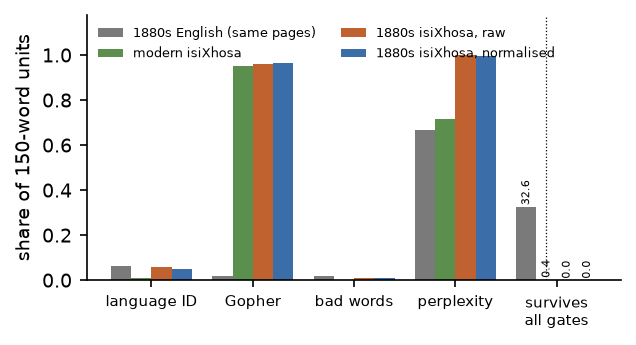
\includegraphics[width=\linewidth]{figures/fig1_cascade.png}
  \caption{\looseness=-1 Share of 150-word windows removed by each gate applied independently, and surviving all four in sequence. Gopher's English stop-word rule removes nearly all isiXhosa regardless of era; only the perplexity gate separates 1880s from modern isiXhosa.}
  \label{fig:cascade}
\end{figure}

\section{Results}
\looseness=-1
\textbf{H1 supported.} 0.0\% [0, 0] of historical isiXhosa windows survive the cascade, against 32.6\% [31.2, 34.3] of the English columns and 0.4\% [0.2, 0.6] of modern isiXhosa (Fig.~\ref{fig:cascade}); paragraph units agree (0.0\% vs 52.6\% English). \textbf{H2 partly supported.} LID is \emph{not} the bottleneck: 92--95\% of historical windows are kept as isiXhosa at every threshold from 0.3 to 0.8, versus 99\% of modern text. The Gopher stop-word rule is a language filter, removing 96\% of historical and 95\% of modern isiXhosa. Swapping in the eight most frequent modern isiXhosa words keeps 90\% of modern but only 71\% of historical windows, because modern function words such as \emph{kwaye} (``and'') are rare in the 1880s (21 per 100k words). The perplexity gate is where history is singled out: it removes 100\% of historical windows but 72\% of modern news (median 3.28 vs 2.52 bits/char). Bad words remove only 1.3\%, but the hits are false positives: surnames (\emph{Dick}, Magistrate \emph{Cumming}), ``Rape'' in seed advertisements, \emph{Exodus xx}, the period spelling \emph{nambla} (modern \emph{namhla}, ``today''), and the single slur, quoted in a report contesting a racist insult against a Black minister.

\textbf{H3: orthography explains a minority of the gap.} Normalisation closes 26\% [22, 29] of the perplexity gap and 18\% [$-4$, 38] of the LID-confidence gap (Fig.~\ref{fig:gap}), yet changes survival by at most 0.2 points: the remaining gap is far above the threshold. Tokenisers spend 1.1--1.6$\times$ more tokens per letter on isiXhosa than on the English columns (e.g.\ XLM-R 0.367 vs 0.273; GPT-2 0.463 vs 0.290), but historical and modern isiXhosa differ by only 1.5--6\% and normalisation moves this by at most 2\%: the tokeniser tax falls on the language, not on its 1880s spelling. In B2, a character LM trained on 1880s text models the (later) 1880s test editions equally well in either spelling (3.10 vs 3.11 bits/raw letter, CIs $\pm$0.04): with in-domain data, spelling is learnable and costs nothing. A purely modern model pays 4.89 bits/letter on 1880s text versus 2.49 on held-out modern text; normalising the test text lowers this to 4.68, closing 9\% of the gap. At a fixed budget, every modern share \emph{hurts} the 1880s test set (3.10$\to$3.43 at 75\% modern), and normalisation's advantage grows with the modern share ($-0.01$, 0.00, 0.01, 0.03, 0.22 bits; H4 weakly supported). Conversely, a model trained only on normalised 1880s text reads modern isiXhosa 0.39 bits/letter better than one trained on raw text (3.58 vs 3.97).

\begin{figure}[h!]
  \centering
  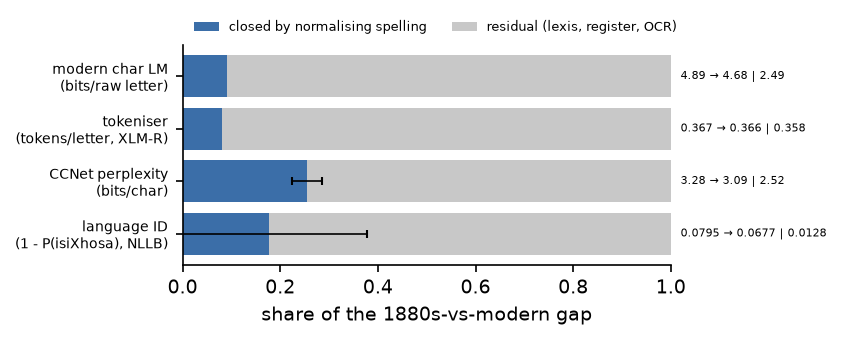
\includegraphics[width=0.95\linewidth]{figures/fig2_gap.png}
  \caption{\looseness=-1 Share of each 1880s-vs-modern gap closed by spelling normalisation (blue; 95\% edition-bootstrap CI where unit-level data exist). Right: raw $\to$ normalised $|$ modern values.}
  \label{fig:gap}
\end{figure}

\section{Discussion}
\looseness=-1
The archive is erased twice over. First by rules that encode English as quality: a stop-word list, and a blocklist that cannot tell a magistrate's surname or the word for ``today'' from obscenity, nor quotation of a slur from its use. Second by a perplexity filter that encodes \emph{modern Wikipedia} as quality, so that period vocabulary (\emph{rulumente}, \emph{ibotile}, \emph{imantyi}), register and OCR noise all count as low quality. Spelling normalisation is a real but small lever, about a quarter of the perplexity gap and less elsewhere, so ``just modernise the spelling'' would not rescue this text; it would also overwrite the historical orthography, itself evidence of how isiXhosa print culture developed. We recommend that curators (i) apply language-appropriate quality rules, (ii) audit blocklist hits rather than dropping documents, and (iii) whitelist or separately score curated heritage collections, keeping original and normalised layers in parallel, with the archive's custodians deciding on reuse \citep{bird2020decolonising,bender2018datastatements}. \textbf{Limitations.} Our filters are re-implementations with published thresholds; the modern control is news and government text, not 19th-century journalism; OCR noise is not separated from lexical change; the normaliser models only aspiration and prefix joining, uses a lexicon that overlaps the perplexity reference, and its gold-set precision is not yet verified by a speaker; the archive's language split was not hand-audited; B2's tuning selected the edge of its grid (order 6, discount 0.9) in every condition, so absolute bits are upper bounds. A failed design choice is reported in the repository: comparing historical paragraphs to whole modern articles (and training the perplexity reference on the control) inflated the gap, which is why we moved to equal-length windows and disjoint reference/control sources.

\section{Acknowledgements (Not in Page Limit)}
TODO: credit the isiXhosa speaker who checks the normalisation gold set.

\section{Contribution Statements (Not in Page Limit)}
TODO: final contribution statement -- all authors must agree on this text (see paper/contribution\_statement/ for the preliminary version).

Do not forget to include the NeurIPS Checklist and the Wits Science Faculty AI Ethics Form.

\bibliographystyle{apacite}
\setlength{\bibleftmargin}{.125in}
\setlength{\bibindent}{-\bibleftmargin}
\bibliography{references}

\end{document}
